%中間審査概要テンプレート ver. 3.0

\documentclass[uplatex,twocolumn,dvipdfmx]{jsarticle}
\usepackage[top=22mm,bottom=22mm,left=22mm,right=22mm]{geometry}
\setlength{\columnsep}{10mm}
\usepackage[T1]{fontenc}
\usepackage{txfonts}
\usepackage[expert,deluxe]{otf}
\usepackage[dvipdfmx,hiresbb]{graphicx}
\usepackage[dvipdfmx]{hyperref}
\usepackage{pxjahyper}
\usepackage{secdot}





%タイトルと学生番号,名前だけ編集すること
\title{\vspace{-5mm}\fontsize{14pt}{0pt}\selectfont 文書自動添削システムによる学生の文書改善履歴の調査}
\author{\normalsize プロジェクトマネジメントコース 矢吹研究室 1442031 氏名 小山隆太郎}
\date{}
\pagestyle{empty}
\begin{document}
\fontsize{10.5pt}{\baselineskip}\selectfont
\maketitle





%以下が本文
\section{背景}
学生が行う研究では,研究だけではなく文書を作成する時間が多い.特に卒業論文は文量も多く,形式も指定されるため,文書校正にかかる労力は大きい.また,自分以外が読んでもわかりやすい文書を書く必要があり,文が長いほど理解が難しくなってしまう場合や,「だから」,「かなり」といった口語が混じり,文書の質が落ちてしまうことがある.

このような状況にRedPen\cite{a}を執筆環境に導入することで,文書の質が向上することが期待されている.RedPenは技術文書をターゲットにした文書自動添削ツールであり,現在もコードの追加,改変が行われている\cite{b}.

\section{目的}
RedPenは学校や会社等の組織のルールに対応できるように設定が柔軟に行える仕様になっている.マシンを用いた文書添削を繰り返し行い,論文向けの添削システムを確立し,文書の質の向上と,作成時間の短縮を図ることを目的とする.

\section{手法}
添削システムに必要な要素を以下の手法で調査する.

\begin{enumerate}
 \item 執筆中の文書を,CI(継続的インテグレーション)サーバを導入し,GitHubへ文書をPushしたときの添削を自動化し,エラー内容を瞬時に確認できるようにする.Pushの度にエラー内容を集める\cite{c}.
 \item 集めた添削結果から添削システムに必要な要素を考察し,RedPenのコードを追加,改変する.
\end{enumerate}

\section{想定される成果物}
個人,複数人プロジェクトで活用できる文書添削システムを構築する.

\section{進捗状況}
矢吹研究室に所属する3年生の課題文の添削を行い,エラー(文中の誤り)数の推移を図\ref{conf}にまとめた.

\begin{figure}[h]
\centering
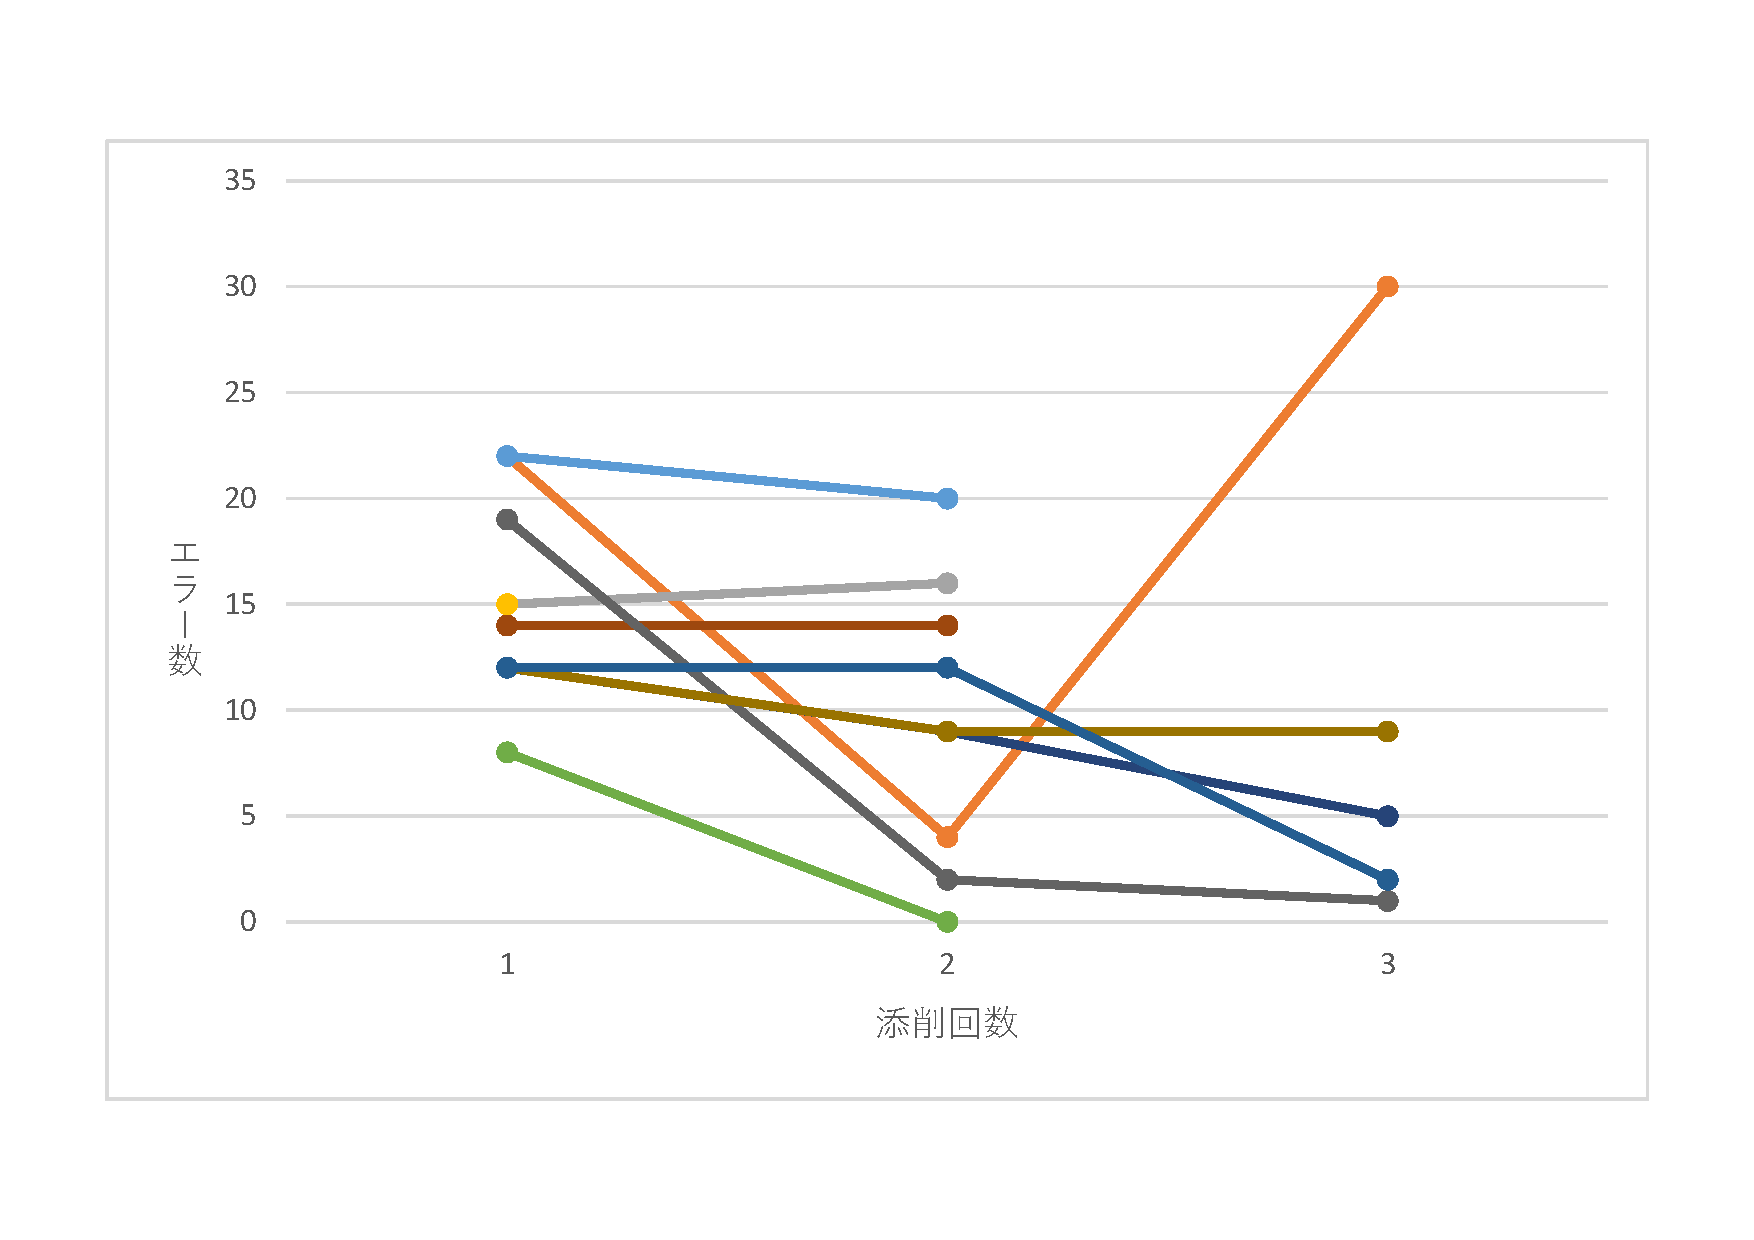
\includegraphics[width=8cm,clip]{images.pdf}
\caption{添削項数の推移}\label{conf}
\end{figure}

エラー内容は,文長が長すぎるために検出されたエラーが多かった.エラー数が減っている文書は,執筆の度に文が短くなる特徴が得られた.

エラー数が減らない文書には,カンマや助詞が多い文が見られた.また,添削システムの設定が不十分であることも要因である.



\section{今後の計画}
論文に適切な文長や表現等の要素を考察し,添削機能の追加,改変を行い機能を実装する.文書作成に利用してもらう.


\bibliographystyle{junsrt}
\bibliography{biblio}%「biblio.bib」というファイルが必要.

\end{document}
